% vim:autoindent:set textwidth=78:

\section{Características de un vistazo}\label{feature_glance}

% when the revision of a section has been finalized, 
% comment out the following line:
%\updatedisclaimer

Después de una primera y sencilla sesión en la Sección \ref{label_getstarted}, ahora
queremos mostrarle una ojeada más detallada de las características de QGIS. 
La mayoría de las características presentadas en los siguientes capítulos se explicarán
y describirán en sus propias secciones más adelante en el manual.

\subsection{Iniciar y detener QGIS}\label{label_startinqgis}

En la Secciónn \ref{samplesession} ya aprendió como iniciar QGIS. Repetiremos
esto aquí y verá que QGIS también proporciona más opciones de línea de órdenes. 

\begin{itemize}
\item \nix{suponiendo que tiene QGIS instalado en el PATH, puede iniciar QGIS
tecleando: \usertext{qgis} en la línea de órdenes o haciendo doble clic sobre el enlace a QGIS 
(o acceso directo) del escritorio.}
\item \win{inicie QGIS usando el menú Inicio o un acceso directo del escritorio, 
o haga doble clic en un archivo de proyecto de QGIS.}
\item \osx{doble clic en el icono de la carpeta Aplicaciones.}
\end{itemize} 

Para detener QGIS, pulse las opciones de menú \{\nix{}\win{Archivo} \osx{QGIS}\} > Salir,
o use el atajo de teclado \keystroke{Ctrl+Q}.

\subsubsection{Opciones de línea de órdenes}\index{command line options}
\label{label_commandline}

\nix QGIS admite un buen número de opciones cuando se inicia desde la línea de 
órdenes. Para obtener la lista de opciones, teclee \usertext{qgis ---help} en la
línea de órdenes.
La sentencia de uso para QGIS es:

\small
\begin{verbatim}
qgis --help
Quantum GIS - 1.1.0-Pan (Unstable) 'Pan (Unstable)'
Quantum GIS (QGIS) is a viewer for spatial data sets, including
raster and vector data.
Usage: qgis [options] [FILES]
  options:
        [--snapshot filename]   emit snapshot of loaded datasets to given file
        [--lang language]       use language for interface text
        [--project projectfile] load the given QGIS project
        [--extent xmin,ymin,xmax,ymax]  set initial map extent
        [--help]                this text

  FILES:
    Files specified on the command line can include rasters,
    vectors, and QGIS project files (.qgs):
     1. Rasters - Supported formats include GeoTiff, DEM
        and others supported by GDAL
     2. Vectors - Supported formats include ESRI Shapefiles
        and others supported by OGR and PostgreSQL layers using
        the PostGIS extension
\end{verbatim}
\normalsize

\begin{Tip} \caption{\textsc{Ejemplo utilizando argumentos en línea de órdenes}}
\qgistip{Puede iniciar QGIS especificando uno o más archivos de datos sobre la
línea de órdenes. Por ejemplo, suponiendo que está en el directorio 
qgis\_sample\_data, podría iniciar QGIS con una capa vectorial 
y un archivo ráster preparados para cargarlos 
en el arranque utilizando la siguiente orden: 
\usertext{qgis ./raster/landcover.img ./gml/lakes.gml}
}
\end{Tip}

\minisec{Opción de línea de órdenes \usertext{---snapshot}}
Esta opción permite crear una captura de pantalla en formato PNG de la vista actual.
Esto puede ser útil cuando se tienen muchos proyectos y se quieren generar capturas de los datos.

Actualmente esto genera un fichero PNG con 800x600 píxeles. Se puede añadir un nombre después de
\usertext{---snapshot}.

\minisec{Opción de línea de órdenes \usertext{---lang}}
En base a su configuración local, QGIS selecciona la localización correcta. Si se quiere 
cambiar el idioma, se puede especificar el código del idioma. Por ejemplo:
\usertext{---lang=it}
arranca QGIS con la localización en italiano. En \url{http://wiki.qgis.org/qgiswiki/TranslatorsCorner}
se proporciona una lista de los idiomas admitidos actualmente con su código.

\minisec{Opción de línea de órdenes \usertext{---project}}
También es posible iniciar QGIS con un proyecto existente. Simplemente añada 
la opción \usertext{---project} seguida del nombre de su proyecto y QGIS se abrirá 
con todas las capas cargadas definidas en el fichero dado.

\minisec{Opción de línea de órdenes \usertext{---extent}}
Para arrancar con una extensión específica del mapa utilice esta opción. Es necesario
añadir los límites en el siguiente orden separados por comas:
\begin{verbatim}
--extent xmin,ymin,xmax,ymax
\end{verbatim}


\subsection{Interfaz Gráfica de Usuario (GUI) de QGIS}\index{main window}
\label{label_qgismainwindow}

Cuando QGIS arranca, se encuentra con la GUI como se muestra abajo
(los números del 1 hasta el 6 en ovalos amarillos señalan las seis áreas principales 
de la interfaz que se describen abajo):

\begin{figure}[ht]
   \begin{center}
   \caption{Interfaz de QGIS con datos de ejemplo de Alaska \nixcaption}
	 \label{fig:startup}
   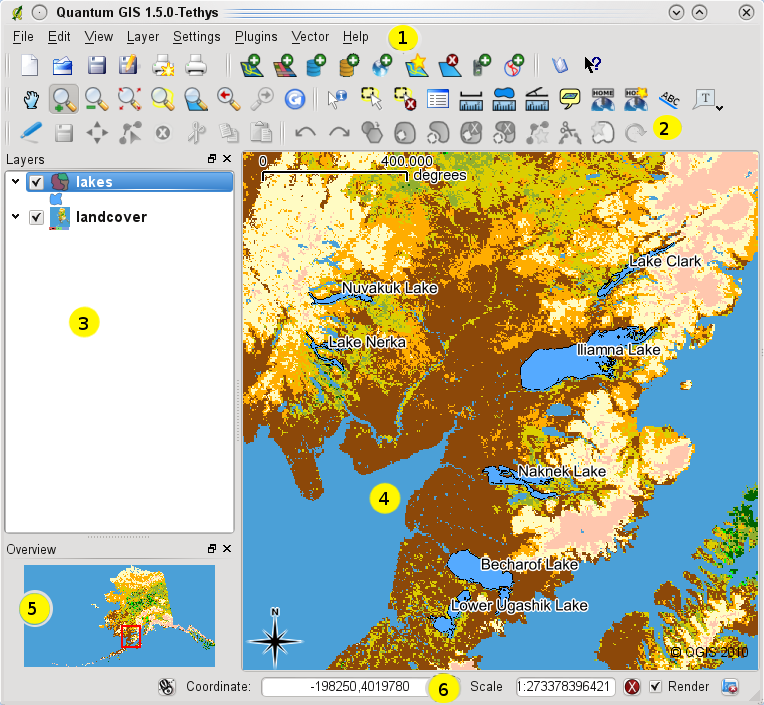
\includegraphics[clip=true, width=17cm]{startup}
\end{center} 
\end{figure}

\textbf{Nota:} La decoración de su ventana (barra de título, etc.) puede aparecer 
distinta dependiendo del sistema operativo y administrador de ventanas.

La Interfaz Gráfica de Usuario (GUI) de QGIS está dividida en seis áreas:

\begin{tabbing}
1. Barra de menús \hspace{3cm}\= 4. Vista del mapa \\
2. Barra de herramientas \hspace{3cm}\> 5. Vista general del mapa \\
3. Capas \hspace{3cm}\> 6. Barra de estado   
\end{tabbing}

Estos seis componentes de la interfaz de QGIS se describen con más detalle
en las siguientes secciones.

\subsubsection{Barra de menús}\label{label_menubar}
\index{menus}

La barra de menús proporciona acceso a varias características de QGIS utilizando 
menús jerárquicos estándar. A continuación se lista el nivel superior de los menús
y un resumen de algunas opciones de menú, junto con los iconos de las herramientas
correspondientes tal como aparece en la barra de herramientas, así como atajos de
teclado. Aunque la mayoría de opciones de menú tiene una herramientas y viceversa,
los menús no están organizados igual que las barras de herramientas. La barra de
herramientas que contiene cada herramienta se indica después de cada opción de menú
como una casilla de verificación. Para más información sobre herramientas y barras
de herramientas, vea la Sección \ref{label_toolbars}.

\begin{tabbing}
\hspace{6.5cm}\=\hspace{3cm}\=\hspace{3.5cm}\= \kill
\hspace{1cm} Opción de menú \> Atajo \> Referencia \> Barra de herramientas\\
\end{tabbing}

\begin{itemize}
\item \mainmenuopt{Archivo}
\begin{tabbing}
\hspace{5.5cm}\=\hspace{3cm}\=\hspace{3.5cm}\= \kill
\dropmenuopttwo{mActionFileNew}{Nuevo proyecto}
	\> \keystroke{Ctrl+N}
	\> Ver sección \ref{sec:projects}
	\> \dropmenucheck{Archivo} \\
\dropmenuopttwo{mActionFileOpen}{Abrir proyecto}
	\> \keystroke{Ctrl+O}
	\> Ver sección \ref{sec:projects}
	\> \dropmenucheck{Archivo} \\
\dropmenuopt{Abrir proyectos recientes}
	\>
	\> Ver sección \ref{sec:projects} \\
\dropmenuopttwo{mActionFileSave}{Guardar proyecto}
	\> \keystroke{Ctrl+S}
	\> Ver sección \ref{sec:projects}
	\> \dropmenucheck{Archivo} \\
\dropmenuopttwo{mActionFileSaveAs}{Guardar proyecto como}
	\> \keystroke{Ctrl+Shift+S}
  \> Ver sección \ref{sec:projects}
	\> \dropmenucheck{Archivo} \\
\dropmenuopttwo{mActionSaveMapAsImage}{Guardar como imagen}
	\>
	\> Ver sección \ref{sec:output} \\
\dropmenuopttwo{mActionFilePrint}{Diseñador de impresión}
	\> \keystroke{Ctrl+P}
	\> Ver sección \ref{label_printcomposer}
	\> \dropmenucheck{Archivo} \\
\dropmenuopttwo{mActionFileExit}{Salir} 
	\> \keystroke{Ctrl+Q} \\
\end{tabbing}

\item \mainmenuopt{Edición}
\begin{tabbing}
\hspace{5.5cm}\=\hspace{3cm}\=\hspace{3.5cm}\= \kill
\dropmenuopttwo{mActionEditCut}{Cortar objetos espaciales} 
	\> \keystroke{Ctrl+X}
	\> Ver sección \ref{sec:edit_existing_layer} 
	\> \dropmenucheck{Digitalización} \\
\dropmenuopttwo{mActionEditCopy}{Copiar objetos espaciales}
	\> \keystroke{Ctrl+C}
	\> Ver sección \ref{sec:edit_existing_layer} 
	\> \dropmenucheck{Digitalización} \\
\dropmenuopttwo{mActionEditPaste}{Pegar objetos espaciales} 
	\> \keystroke{Ctrl+V}
	\> Ver sección \ref{sec:edit_existing_layer} 
	\> \dropmenucheck{Digitalización} \\
\dropmenuopttwo{mActionCapturePoint}{Añadir punto}
	\> \keystroke{.}
	\> Ver sección \ref{sec:edit_existing_layer} 
	\> \dropmenucheck{Digitalización} \\
\dropmenuopttwo{mActionCaptureLine}{Añadir línea}
	\> \keystroke{/}
	\> Ver secciónn \ref{sec:edit_existing_layer} 
	\> \dropmenucheck{Digitalización} \\
\dropmenuopttwo{mActionCapturePolygon}{Añadir polígono}
	\> \keystroke{Ctrl+/}
	\> Ver sección \ref{sec:edit_existing_layer} 
	\> \dropmenucheck{Digitalización} \\
Y otros elementos del menú Edición
	\>
	\> Ver sección \ref{sec:edit_existing_layer} 
	\> \dropmenucheck{Digitalización} \\
%\dropmenuopt{Move Feature}
%	\> \> \dropmenucheck{Edit} \\
%\dropmenuopt{Split Features}
%	\> \> \dropmenucheck{Edit} \\
%\dropmenuopt{Delete Selected}
%	\> \> \dropmenucheck{Edit} \\
%\dropmenuopt{Add Vertex}
%	\> \> \dropmenucheck{Edit} \\
%\dropmenuopt{Move Vertex}
%	\> \> \dropmenucheck{Edit} \\
%\dropmenuopt{Delete Vertex}
%	\> \> \dropmenucheck{Edit} \\
%\dropmenuopt{Add Ring}\footnote{New since v0.9} 
%	\>
%	\> \dropmenucheck{Edit} \\
%\dropmenuopt{Add Island} \footnotemark[\value{footnote}] 
%	\>
%	\> \dropmenucheck{Edit} \\
\end{tabbing}


\item \mainmenuopt{Ver}
\begin{tabbing}
\hspace{5.5cm}\=\hspace{3cm}\=\hspace{3.5cm}\= \kill
\dropmenuopttwo{mActionPan}{Desplazar mapa}
	\>
	\> \> \dropmenucheck{Navegación de mapas} \\
\dropmenuopttwo{mActionZoomIn}{Acercar zum}
	\> \keystroke{Ctrl++}
	\> \> \dropmenucheck{Navegación de mapas} \\
\dropmenuopttwo{mActionZoomOut}{Alejar zum}
	\> \keystroke{Ctrl+-}
	\> \> \dropmenucheck{Navegación de mapas} \\
\dropmenuopttwo{mActionSelect}{Seleccionar objetos espaciales}
	\>
	\> \> \dropmenucheck{Atributos} \\
\dropmenuopttwo{mActionIdentify}{Identificar objetos espaciales}
	\> \keystroke{I}
	\> \> \dropmenucheck{Atributos} \\
\dropmenuopttwo{mActionMeasure}{Regla}
	\> \keystroke{M}
	\> \> \dropmenucheck{Atributos} \\
\dropmenuopttwo{mActionMeasureArea}{Medir áreas}
	\> \keystroke{J}
	\> \> \dropmenucheck{Atributos} \\
\dropmenuopttwo{mActionOpenTable}{Zum general}
	\> \keystroke{F}
	\> \> \dropmenucheck{Navegación de mapas} \\
\dropmenuopttwo{mActionZoomToLayer}{Zum a la capa}
	\>
	\> \> \dropmenucheck{Navegación de mapas} \\
\dropmenuopttwo{mActionZoomToSelected}{Zum a la selección}
	\> \keystroke{Ctrl+J}
	\> \> \dropmenucheck{Navegación de mapas} \\
\dropmenuopttwo{mActionZoomLast}{Zum anterior}
	\>
		\> \> \dropmenucheck{Navegación de mapas} \\
\dropmenuopttwo{mActionZoomNext}{Zum siguiente}
	\>
	\> \> \dropmenucheck{Navegación de mapas} \\
\dropmenuopt{Zum al tamaño real}
	\>
	\> \>  \\
\dropmenuopttwo{mActionMapTips}{Avisos del mapa}
	\>
	\> \> \dropmenucheck{Atributos} \\
\dropmenuopttwo{mActionNewBookmark}{Nuevo marcador}
	\> \keystroke{Ctrl+B}
	\> Ver sección \ref{sec:bookmarks} 
\> \dropmenucheck{Atributos} \\
\dropmenuopttwo{mActionShowBookmarks}{Mostrar marcadores}
	\> \keystroke{B}
	\> Ver sección \ref{sec:bookmarks} 
	\> \dropmenucheck{Atributos} \\
\dropmenuopttwo{mActionDraw}{Actualizar}
	\> \keystroke{Ctrl+R}
	\> \> \dropmenucheck{Navegación de mapas} \\
\end{tabbing}

\item \mainmenuopt{Capa}
\begin{tabbing}
\hspace{5.5cm}\=\hspace{3cm}\=\hspace{3.5cm}\= \kill
\dropmenuopttwo{mActionNewVectorLayer}{Nueva capa vectorial}
	\> \keystroke{N}
	\>          	
	Ver sección \ref{sec:create shape}
	\> \dropmenucheck{Administrar capas} \\
\dropmenuopttwo{mActionAddNonDbLayer}{Añadir capa vectorial}       
	\> \keystroke{V}
	\>          	
	Ver sección \ref{label_workingvector}
	\> \dropmenucheck{Archivo} \\
\dropmenuopttwo{mActionAddRasterLayer}{Añadir capa ráster}       
	\> \keystroke{R}
	\>          	
	Ver sección \ref{label_raster}
	\> \dropmenucheck{Archivo} \\
\dropmenuopttwo{mActionAddLayer}{Añadir capa PostGIS}      
	\> \keystroke{D}
	\>          	
	Ver sección \ref{label_postgis}
	\> \dropmenucheck{Archivo} \\
\dropmenuopttwo{mActionAddWmsLayer}{Añadir capa WMS}          
	\> \keystroke{W}
	\>          	
	Ver sección \ref{sec:ogc-wms}
	\> \dropmenucheck{Archivo} \\
\dropmenuopttwo{mActionOpenTable}{Abrir tabla de atributos}
	\> \>
	\> \dropmenucheck{Atributos} \\
\dropmenuopttwo{mActionToggleEditing}{Conmutar edición}
	\> \>
	\> \dropmenucheck{Digitalización} \\
\dropmenuopt{Guardar como archivo shape}
	\\
\dropmenuopt{Guardar la selección como archivo shape}
	\\
\dropmenuopttwo{mActionRemoveLayer}{Eliminar capa}
	\> \keystroke{Ctrl+D}
	\>          	
	\> \dropmenucheck{Administrar capas} \\
\dropmenuopt{Propiedades}
	\\
\dropmenuopttwo{mActionInOverview}{Añadir a la vista general}
	\> \keystroke{O}
	\>          	
	\> \dropmenucheck{Administrar capas} \\
\dropmenuopttwo{mActionAddAllToOverview}{Añadir todo a la vista general}
	\> \keystroke{+}
	\>          	
	\\
\dropmenuopttwo{mActionRemoveAllFromOverview}{Eliminar todo de la vista general}
	\> \hspace{1cm}\keystroke{-}
	\>          	
	\\
\dropmenuopttwo{mActionHideAllLayers}{Ocultar todas las capas}
	\> \keystroke{H}
	\>          	
	\> \dropmenucheck{Administrar capas} \\
\dropmenuopttwo{mActionShowAllLayers}{Mostrar todas las capas}
	\> \keystroke{S}
	\>          	
	\> \dropmenucheck{Administrar capas} \\
\end{tabbing}

\item \mainmenuopt{Configuración}
\begin{tabbing}
\hspace{5.5cm}\=\hspace{3cm}\=\hspace{3.5cm}\= \kill
\dropmenuopt{Paneles}  
	\>           
	\>          	
	\\
\dropmenuopt{Barras de herramientas}  
	\>           
	\>          	
	\\
\dropmenuopt{Conmutar el modo de pantalla completa}  
	\>
	\>          	
	\\
\dropmenuopttwo{mActionProjectProperties}{Propiedades del proyecto}  
	\> \keystroke{P}
	\>          	
	Ver sección \ref{sec:projects}
	\\
\dropmenuopttwo{mActionCustomProjection}{SRC personalizado}   
\> \>          	
Ver sección \ref{sec:customprojections}
	\\
\dropmenuopttwo{mActionOptions}{Opciones}             
\> \>          	
Ver sección \ref{subsec:gui_options}
	\\
\end{tabbing}

\item \mainmenuopt{Complementos} - (Se añaden más elementos de menú a medida que se cargan complementos.)
\begin{tabbing}
\hspace{5.5cm}\=\hspace{3cm}\=\hspace{3.5cm}\= \kill
\dropmenuopttwo{mActionShowPluginManager}{Administrador de complementos}          	   
\> \>          	
Ver sección \ref{sec:managing_plugins}
	\dropmenucheck{Complementos}\\
\end{tabbing}          	

\item \mainmenuopt{Ayuda}
\begin{tabbing}
\hspace{5.5cm}\=\hspace{3cm}\=\hspace{3.5cm}\= \kill
\dropmenuopttwo{mActionHelpContents}{Contenidos de la ayuda}
	\> \keystroke{F1}
	\>           	
	\> \dropmenucheck{Ayuda}\\
\dropmenuopttwo{mActionQgisHomePage}{Página web de QGIS}
	\> \keystroke{Ctrl+H}
	\>          	
	\\
\dropmenuopttwo{mActionCheckQgisVersion}{Comprobar versión de QGIS}
	\\
\dropmenuopttwo{mActionHelpAbout}{Acerca de}
	\\
\end{tabbing}

\end{itemize}

%See Appendix \ref{app_menu} for complete descriptions of the menu items.

\subsubsection{Barras de herramientas}\label{label_toolbars}
\index{toolbars}

Las barras de herramientas proporcionan acceso a la mayoría de las mismas funciones que los menús,
así como a herramientas adicionales para interactuar con el mapa. Cada elemento de barra de herramientas tiene
una ayuda emergente disponible. Mantenga el ratón sobre el elemento y se mostrará una breve descripción del
propósito de la herramienta.

Cada barra de menú se puede mover de acuerdo a sus necesidades. Además, cada
barra de menú se puede desactivar usando el menú contextual del botón derecho del ratón manteniendo el ratón sobre las barras de herramientas.

\begin{Tip}
\caption{\textsc{Restaurar las barras de herramientas}} \index{layout!toolbars}
\qgistip{Si ha ocultado accidentalmente todas sus barras de herramientas, puede recuperarlas
mediante la opción de menú \mainmenuopt{Configuración} > \dropmenuopt{Barras de herramientas}.}
\end{Tip}

\subsubsection{Capas}\label{label_legend}
\index{legend}

El área de las capas se usa para establecer la visibilidad y el orden vertical de las capas.
El orden vertical significa que las capas colocadas cerca de la parte superior se dibujan
sobre
las capas mostradas más abajo. La casilla de verificacion de cada entrada de la leyenda
se puede usar para mostrar u ocultar la capa.\index{layer!visibility}

Las capas se pueden agrupar en la ventana Capas añadiendo un grupo de capas y arrastrando las capas 
dentro del grupo. Para ello, mueva el puntero del ratón a la ventana Capas, haga clic derecho y seleccione \dropmenuopt{Añadir grupo}. 
Aparecerá una carpeta nueva. Ahora arrastre las capas sobre el símbolo de la carpeta. A continuación es posible
conmutar la visibilidad de todas las capas del grupo con un clic. Para sacar las capas del grupo, mueva 
el puntero del ratón al símbolo de la capa, haga clic derecho y seleccione \dropmenuopt{Subir el elemento al nivel superior}. 
Para poner un nombre a la carpeta, seleccione \dropmenuopt{Cambiar nombre} en el menú del botón derecho del grupo.

El contenido del menú contextual del botón derecho depende de si la capa sobre la que se pasa el
ratón es ráster o vectorial. Para las capas vectoriales de GRASS no está disponible la opción \dropmenuopt{Conmutar edición}.
Vea la sección \ref{grass_digitising} para información sobre la edición de capas vectoriales de GRASS. 

\begin{itemize}

\item \textbf{Menú del botón derecho del ratón para capas ráster}
\begin{itemize}
\item \dropmenuopt{Zum a la extensión de la capa}
\item \dropmenuopt{Zum a la mejor escala (100\%)}
\item \dropmenuopt{Mostrar en la vista general}
\item \dropmenuopt{Eliminar}
\item \dropmenuopt{Propiedades}
\item \dropmenuopt{Cambiar nombre}
\item \dropmenuopt{Añadir grupo}
\item \dropmenuopt{Expandir todo}
\item \dropmenuopt{Comprimir todo}
\item \dropmenuopt{Mostrar grupos de archivos}
\end{itemize}

\item \textbf{Menú del botón derecho del ratón para capas vectoriales}
\begin{itemize}
\item \dropmenuopt{Zum a la extensión de la capa}
\item \dropmenuopt{Mostrar en la vista general}
\item \dropmenuopt{Eliminar}
\item \dropmenuopt{Abrir tabla de atributos}
\item \dropmenuopt{Conmutar edición (no disponible para capas de GRASS)}
\item \dropmenuopt{Guardar como archivo shape}
\item \dropmenuopt{Guardar selección como archivo shape}
\item \dropmenuopt{Propiedades}
\item \dropmenuopt{Subir el elemento al nivel superior}
\item \dropmenuopt{Cambiar nombre}
\item \dropmenuopt{Añadir grupo}
\item \dropmenuopt{Expandir todo}
\item \dropmenuopt{Comprimir todo}
\item \dropmenuopt{Mostrar grupos de archivos}
\end{itemize}

\item \textbf{Menú del botón derecho del ratón para grupos de capas} 
\begin{itemize}
\item \dropmenuopt{Eliminar}
\item \dropmenuopt{Cambiar nombre}
\item \dropmenuopt{Añadir grupo}
\item \dropmenuopt{Expandir todo}
\item \dropmenuopt{Comprimir todo}
\item \dropmenuopt{Mostrar grupos de archivos}
\end{itemize}

\end{itemize}

Si varias fuentes de datos vectoriales tienen el mismo tipo de vector y el mismo tipo de atributos, su
simbología se puede agrupar. Esto significa que si cambia la simbología de una fuente de datos, 
las otras automáticamente tendrán también la nueva simbología. Para agrupar simbologías, abra 
el menú del botón derecho de la ventana Capas y seleccione \dropmenuopt{Mostrat grupos de archivos}. Aparecerán los 
grupos de archivos de las capas. Ahora es posible arrastrar un archivoo de un grupo de archivos a otro. Si se hace esto, 
las simbologías se agrupan. Tenga en cuenta que QGIS sólo permite arrastrar si las dos capas pueden compartir
la simbología (misma geometría vectorial y mismos atributos). 

%% isn't included in Titan anymore, except for an "toggle overview"
%Each legend entry can show the following mini icons:
%
%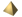
\includegraphics[width=0.7cm]{pyramid} This is a raster
%that has pyramids built for it to improve rendering efficiency (see
%Section \ref{raster_pyramids}).\\
%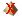
\includegraphics[width=0.7cm]{no_pyramid} This is a
%raster that has no pyramid layers (see Section \ref{raster_pyramids}).\\
%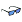
\includegraphics[width=0.7cm]{inoverview} This layer is
%shown in the overview map area as well as in the main map window.\\
%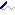
\includegraphics[width=0.7cm]{editable} This is a vector
%layer that is currently enabled for editing.\\

\subsubsection{Vista del mapa}\label{label_mapview}
\index{map!view}

Este es el «objetivo final» de QGIS - ¡los mapas se muestran en este área! El mapa que se visualice en esta 
ventana dependerá de las capas vectoriales y ráster que se hayan seleccionado para cargar (vea las secciones que siguen 
para más información sobre cómo cargar capas). Las vista del mapa se puede desplazar (moviendo el foco de 
visualización del mapa a otra región) y se puede acercar y alejar el zum. Se pueden realizar otras operaciones 
sobre el mapa como se indica en la descripción de las barras de herramientas más arriba. La vista del mapa y la 
ventana Capas están íntimamente relacionadas – los mapas de la vista reflejan los cambios que se hacen en el área de las Capas. 

\begin{Tip}\caption{\textsc{Hacer zum sobre el mapa con la rueda del ratón}}\index{zoom!mouse wheel}
\qgistip{Se puede usar la rueda del ratón para acercar o alejar el zum sobre el mapa. Sitúe el cursor del ratón 
dentro del área del mapa y gire la rueda hacia delante para acercar el zum y hacia atrás para alejarlo. El 
cursor del ratón es el centro sobre el que se hace zum. Puede personalizar el comportamiento del zum con la 
rueda del ratón usando la pestaña \tab{Herramientas de mapa} bajo el menú \mainmenuopt{Configuración} >\dropmenuopt{Opciones}.  }
\end{Tip}

\begin{Tip}\caption{\textsc{Desplazar el mapa con las flechas de desplazamiento y la barra espaciadora}}\index{pan!arrow keys}
\qgistip{Puede usar las flechas de desplazamiento para desplazar el mapa. Sitúe el cursor del ratón 
dentro del área del mapa y pulse la flecha derecha para desplazarse al Este, la flecha izquierda 
para desplazarse al Oeste, la flecha arriba para desplazarse al Norte y la  flecha abajo para desplazarse al Sur. 
También puede desplazar el mapa usando la barra espaciadora: simplemente mueva el ratón mientras mantiene pulsada la barra espaciadora .
}
\end{Tip}

\subsubsection{Vista general}\label{label_mapoverview}
\index{map!overview}

La vista general proporciona una vista de toda la extensión de las capas añadidas al mapa. Dentro de la 
vista hay un rectángulo que muestra la extensión actual del mapa. Esto permite determinar rápidamente que área 
del mapa se está viendo actualmente. Tenga en cuenta que las etiquetas no se visualizan en la vista general, 
incluso aunque las capas se hayan configurado para ser etiquetadas. Puede añadir una sola capa a la vista general 
pulsando con el botón derecho sobre ella en la ventana capas y seleccionando \checkbox{Mostrar en la vista general}. 
También puede añadir o quitar todas las capas de la vista general usando las herramientas de la vista general en 
la barra de herramientas.

Si coge y arrastra el rectángulo rojo de la vista general que muestra la extensión actual, la vista 
del mapa se actualizará conforme se desplace.

\subsubsection{Barra de estado}\label{label_statusbar}

La barra de estado muestra su posición actual en las coordenadas del mapa (ej.: 
metros o grados decimales) a medida que el puntero del ratón se mueve por la vista del mapa. 
A la izquierda de la visualización de las coordenadas hay un pequeño botón que alterna entre 
mostrar las coordenadas de la posición o la extensión de la 
vista del mapa a medida que desplaza el mapa o modifica el nivel del zum. 

Una barra de progreso en la barra de estado muestra el progreso de la representación de cada capa que se está 
dibujando en la vista del mapa. En algunos casos, tales como la recopilación de estadísticas en capas ráster, 
la barra de progreso se usará para mostrar el estado de operaciones prolongadas.

Si hay disponible un complemento nuevo o una actualización de complementos, verá un mensaje en la barra de estado. 
Puede pulsar en el mensaje para abrir el Administrador de complementos e instalar o actualizar los complementos.
En la parte derecha de la barra de estado hay una pequeña casilla de verificación 
que se puede usar para 
evitar temporalmente que se representen las capas en la vista del mapa (vea la Sección 
\ref{subsec:redraw_events} más abajo). 
En el extremo derecho de la barra de estado hay un icono de un proyector. 
Pulsando en él se abren 
las propiedades del proyecto actual.

\begin{Tip}\caption{\textsc{Calcular la escala correcta de su vista del mapa}}\index{scale!calculate}
\qgistip{Cuando arranca QGIS, la unidad predeterminada son grados y ésto le dice a QGIS 
que cualquier coordenada
en sus capas está en grados. Para conseguir valores de escala correctos, 
puede o cambiar esto a 
metros manualmene en la pestaña \tab{General} bajo \mainmenuopt{Configuración} >\dropmenuopt{Propiedades 
del proyecto} o puede seleccionar un Sistema de Referencia de Coordenadas (SRC) del proyecto pulsando en el 
icono \toolbtntwo{mIconProjectionEnabled}{Proyector} en la esquina inferior derecha de la barra de estado. En el 
último caso, las unidades se fijan a lo que especifique la proyección del proyecto, por ejemplo '+units=m'.
}
\end{Tip}

\subsection{Representación}\label{subsec:redraw_events}\index{rendering}

Por omisión, QGIS representa todas las capas visibles cada vez que la vista del mapa se debe refrescar. Los eventos 
que desencadenan un refresco de la vista del mapa incluyen:

\begin{itemize}
\item Añadir una capa.
\item Desplazamiento o zum.
\item Redimensionar la ventana de QGIS.
\item Cambiar la visibilidad de una o más capas.
\end{itemize}

QGIS permite controlar el proceso de representación de distintas formas.

\subsubsection{Representación dependiente de la escala}\index{rendering!scale dependent}
\label{label_scaledepend}

La representación dependiente de la escala permite especificar las escalas máxima y mínima a las que una capa será 
visible. Para establecer la representación dependiente de la escala, abra el diálogo  \dialog{Propiedades} haciendo 
doble clic sobre una capa en la ventana Capas. En la pestaña \tab{General}, establezca la escala mínima y máxima y luego marque la casilla \checkbox{Utilizar 
representación dependiente de la escala}.

Puede determinar los valores de escala haciendo zum primero al nivel que quiera usar y anotando el valor de la 
escala mostrado en la barra de estado de QGIS.\index{scale}

\subsubsection{Controlar la representación del mapa}\label{label_controlmap}

La representación del mapa se puede controlar de las siguientes formas:

\minisec{a) Suspender la representación}\index{rendering!suspending}
\label{label_suspendrender}

Para suspender la representación, desmarque la casilla \checkbox{Representar} en la esquina inferior derecha de la 
barra de estado. Cuando la casilla \checkbox{Representar} no está marcada, QGIS no redibuja la vista del mapa en 
respuesta a ninguno de los eventos descritos en la Sección
\ref{subsec:redraw_events}. Entre los ejemplos de cuándo puede desear suspender la representación se incluyen:

\begin{itemize}
\item Añadir muchas capas y simbolizarlas antes de que se dibujen.
\item Añadir una o más capas grandes y establecer la dependencia de la escala antes de dibujarlas.
\item Añadir una o más capas grandes y hacer zum a una zona específica antes de dibujarla.
\item Cualquier combinación de las anteriores.
\end{itemize}

Marcar la casilla \checkbox{Representar} activa la representación y desencadena el refresco inmediato de la vista del mapa.

\minisec{b) Establecer opción al añadir capas}\label{label_settinglayer}
\index{rendering!options}\index{layers!initial visibility}

Se puede establecer una opción para que siempre se carguen las capas nuevas sin dibujarlas. Esto
significa que las capas se añadirán al mapa, pero su casilla de verificación de visualización en la ventana Capas estará 
desmarcada por omisión. Para establecer esta opción, seleccione la opción de menú \mainmenuopt{Configuración} > \dropmenuopt{Opciones}
y pulse en la pestaña \tab{Representación}. Desmarque la casilla \checkbox{Por omisión, las nuevas capas añadidas 
al mapa se deben visualizar}. Cualquier capa que añada al mapa estará desactivada (invisible) por omisión.

%\minisec{Stopping Rendering}\index{rendering!halting}
%\label{label_stoprender}
%
%To stop the map drawing, press the ESC key. This will halt the refresh of
%the map canvas and leave the map partially drawn. It may take a bit of time
%between pressing ESC and the time the map drawing is halted.
%
%\textbf{NOTE}: It is currently not possible to stop rendering - this was disabled 
%in qt4 port because of User Interface (UI) problems and crashes.

\minisec{c) Actualizar la vista del mapa durante la representación}
\label{label_updatemap}\index{rendering!update during drawing}

Puede establecer una opción para actualizar la vista del mapa a medida que se dibujan los objetos espaciales. Por
omisión, QGIS no muestra ningún objeto espacial de una capa hasta que toda la capa se ha renderizado. 
Para actualizar la vista a medida que se leen los objetos espaciales, seleccione la opción de menú
\mainmenuopt{Configuración} > \dropmenuopt{Opciones} y pulse en la pestaña \tab{Representación}. 
Establezca el número de objetos espaciales a un valor adecuado para actualizar la vista durante la representación.
Establecer un valor de 0 desactiva la actualización durante la representación (es el valor predeterminado).
Establecer un valor demasiado bajo dará como resultado un rendimiento bajo, ya que el lienzo del mapa se está
actualizando continuamente mientras se leen los objetos espaciales. Se sugiere un valor de 500 para empezar. 

\minisec{d) Influir en la calidad de la representación}
\label{label_renderquality}\index{rendering!quality}

Para influir en la calidad de la representación del mapa tiene tres opciones. Seleccione la opción de menú
\mainmenuopt{Configuración} > \dropmenuopt{Opciones}, pulse en la pestaña 
\tab{Representación} 
y marque o desmarque las siguientes casillas:

\begin{itemize}
\item \checkbox{Hacer que las líneas se muestren menos quebradas a expensas del rendimiento de la representación}
\item \checkbox{Solucionar problemas con polígonos rellenados incorrectamente}
\item \checkbox{Redibujar el mapa continuamente mientras se desplaza el separador entre mapa y leyenda}
\end{itemize}


\subsection{Medir}\label{sec:measure}\index{measure}

Las mediciones funcionan únicamente en sistemas de coordenadas proyectadas (ej.: UTM). Si el mapa cargado
está definido con un sistema de coordenadas geográficas (latitud/longitud), los resultados de las medidas
de líneas o polígonos serán incorrectos. Para solucionarlo necesita establecer un sistema de coordenadas
adecuado (vea la sección~\ref{label_projections}).

\subsubsection{Medir longitudes y áreas}\index{measure:line length}\index{measure:areas}
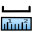
\includegraphics[width=0.7cm]{mActionMeasure} 
QGIS también es capaz de medir distancias reales entre puntos dados, de acuerdo con el elipsoide definido.
Para configurar esto, seleccione la opción de menú \mainmenuopt{Configuración} > \dropmenuopt{Opciones}, 
pulse en la pestaña \tab{Herramientas de mapa} y seleccione el elipsoide adecuado. La herramienta le 
permite entonces pulsar puntos en el mapa. La longitud de cada segmento se muestra en la ventana de medidas
así como el total. Para detener la medición, pulse el botón derecho del ratón. \\
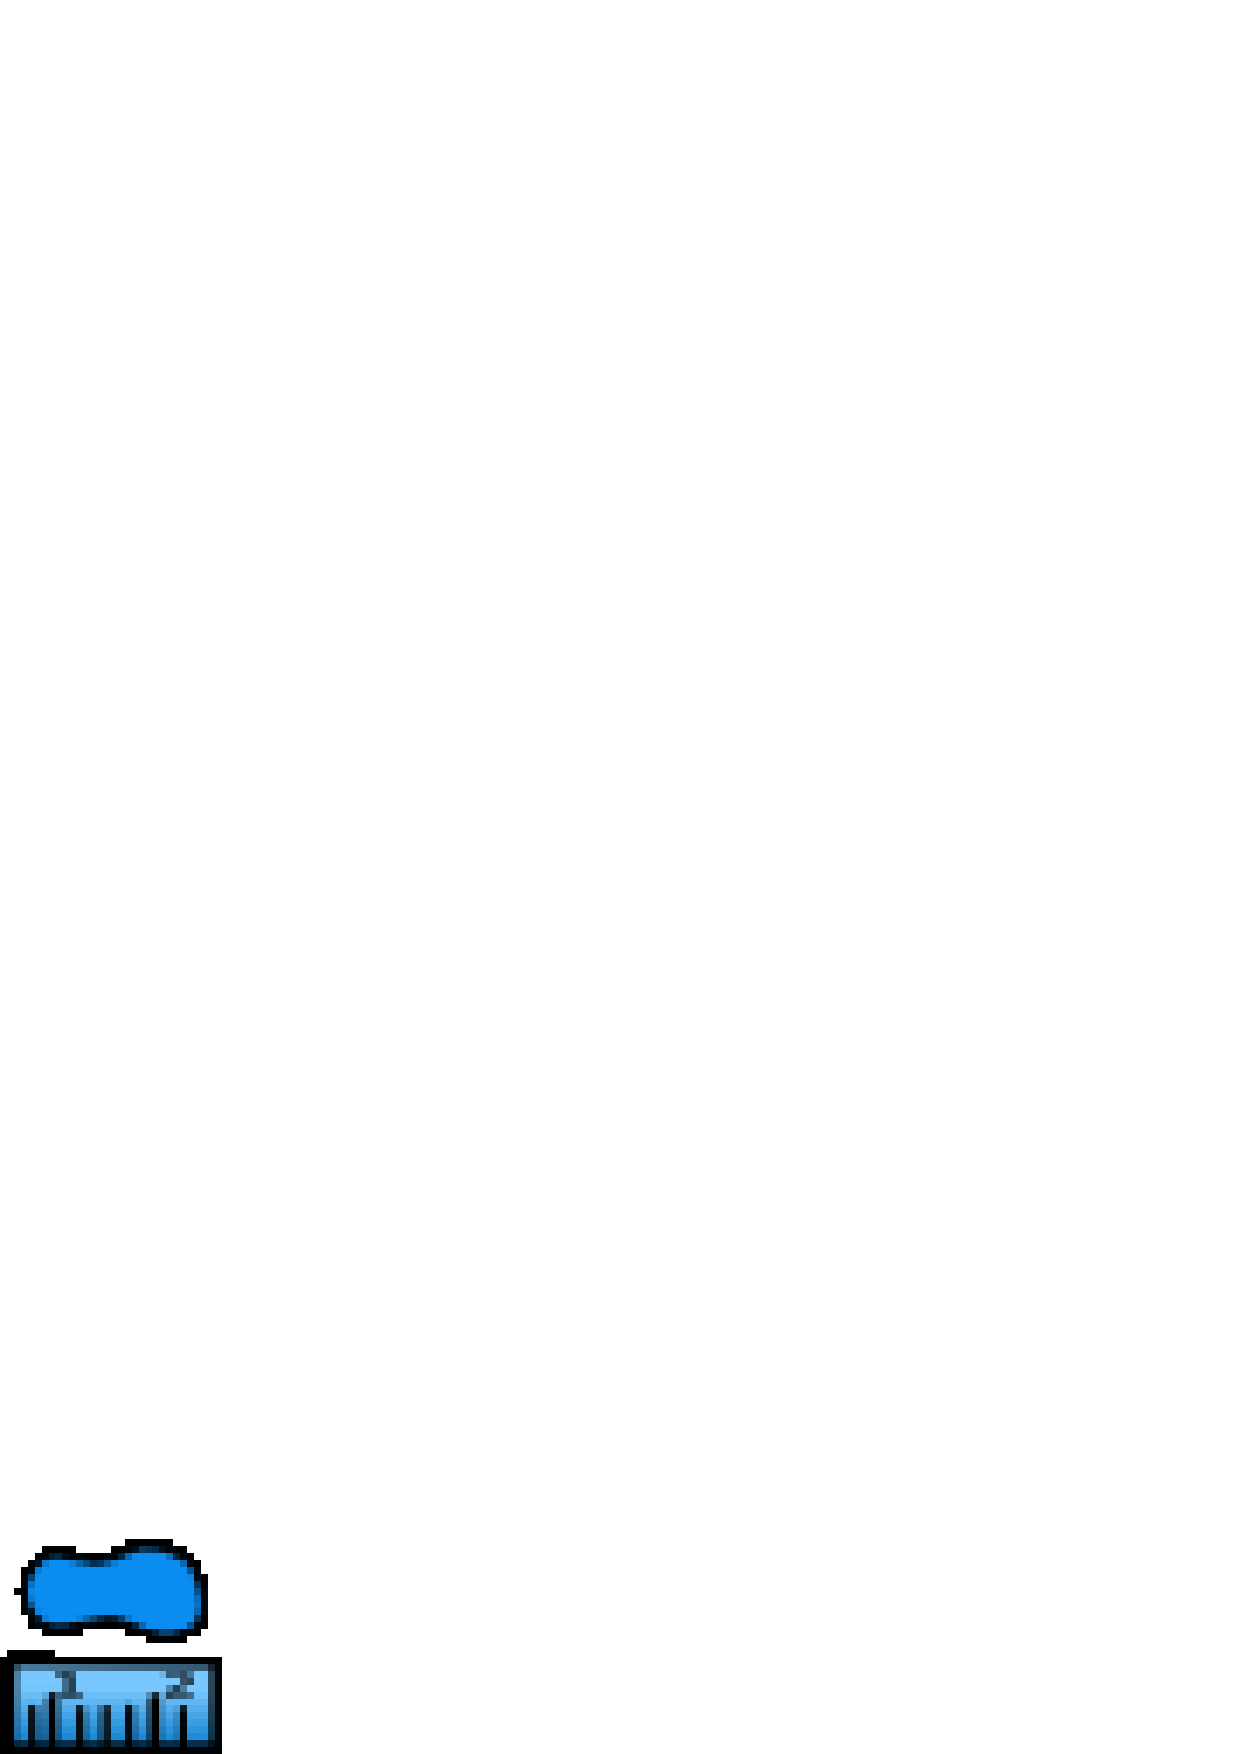
\includegraphics[width=0.7cm]{mActionMeasureArea} También se pueden medir áreas. 
La ventana muestra el área acumulada. 

\begin{figure}[h]
\caption{Herramientas de medida en acción \nixcaption} \label{fig:measure}
\centering
   \subfigure[Medir líneas] {\label{subfig:measure_line}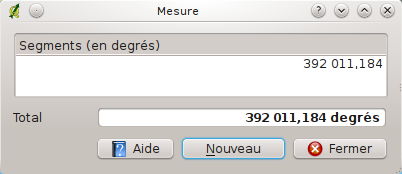
\includegraphics[clip=true, width=0.3\textwidth]{measure_line}}\goodgap
   \subfigure[Medir áreas]{\label{subfig:measure_area}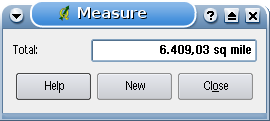
\includegraphics[clip=true, width=0.3\textwidth]{measure_area}}
\end{figure}

\subsection{Proyectos}\label{sec:projects}\index{projects}

El estado de su sesión de QGIS se considera un proyecto. QGIS
trabaja en un proyecto en cada momento. Las configuraciones se considera que son
por proyecto o como predeterminadas para nuevos proyectos (vea 
la sección \ref{subsec:gui_options}). QGIS puede guardar el estado de su entorno de trabajo
en un archivo de proyecto usando las opciones de menú 
\mainmenuopt{Archivo} > \dropmenuopttwo{mActionFileSave}{Guardar proyecto}
o \mainmenuopt{Archivo} > \dropmenuopttwo{mActionFileSaveAs}{Guardar proyecto como}.

Cargue proyectos guardados en una sesión de QGIS usando 
\mainmenuopt{Archivo} > \dropmenuopttwo{mActionFileOpen}{Abrir proyecto}
o \mainmenuopt{Archivo} > \dropmenuopt{Abrir proyectos recientes}.
Si desea limpiar su sesión y comenzar una en blanco, seleccione
\mainmenuopt{Archivo} > \dropmenuopttwo{mActionFileNew}{Nuevo proyecto}.
Cualquiera de estas opciones de menú le pedirá que guarde el proyecto activo si se han
realizado cambios desde que se abrió o se guardó por última vez.

El tipo de información guardada en un archivo de proyecto incluye:

\begin{itemize}
\item Capas añadidas.
\item Propiedades de las capas, incluyendo la simbología.
\item Proyección de la vista del mapa.
\item Última extensión visualizada.
\end{itemize}

El proyecto se guarda en un archivo con formato XML, así que es posible editarlo
fuera de QGIS si sabe lo que está haciendo. El formato de archivo se ha actualizado
varias veces en relación con versiones anteriores de QGIS. Los archivos de proyectos 
de versiones anteriores de QGIS puede que ya no funcionen correctamente. Para hacerle
consciente de esto, en la pestaña \tab{General} bajo \mainmenuopt{Configuración} > \dropmenuopt{Opciones} 
puede seleccionar la casilla \checkbox{Avisar cuando se abra
un proyecto guardado con una versión anterior de QGIS}.

\subsection{Salida}\label{sec:output}\index{output!save as image!print composer!quick print}
Hay varias formas para generar una salida de su sesión de QGIS.
Ya hemos visto una en la sección \ref{sec:projects}: guardar como un archivo de proyecto. 
Aquí hay una muestra de otras formas de producir archivos de salida:
\begin{itemize}
\item Opción de menú \dropmenuopttwo{mActionSaveMapAsImage}{Guardar como imagen} abre un
diálogo de archivo donde seleccionar el nombre, ruta y tipo de imagen (formato PNG o JPG). Desde esta
versión, se guarda un archivo de georreferenciación con extensión PNGW o JPGW en la misma carpeta.
\item Opción de menú \dropmenuopttwo{mActionFilePrint}{Diseñador de impresión} abre un
diálogo en el que puede organizar e imprimir la vista del mapa actual (vea la
sección~\ref{label_printcomposer}).
\end{itemize}


\subsection{Opciones de la Interfaz}
\label{subsec:gui_options}

\includegraphics[width=0.7cm,clip=true]{mActionOptions} 
Se pueden seleccionar algunas opciones básicas de QGIS usando el diálogo \dialog{Opciones}.
Seleccione la opción de menú \mainmenuopt{Configuración} >
 \dropmenuopttwo{mActionOptions}{Opciones}. Las pestañas en las que puede optimizar
sus opciones son:

\minisec{Pestaña General}

\begin{itemize}
\item \checkbox{Preguntar si guardar cambios en el proyecto cuando sea necesario}
\item \checkbox{Avisar cuando se abra un proyecto guardado con una versión anterior de QGIS}
\item \checkbox{Cambiar el color de selección y de fondo}
\item Cambiar el tema de iconos (elija entre predeterminado (default), classic, gis y nkids)
\item \checkbox{Comenzar el nombre de las capas con mayúsculas en la leyenda}
\item \checkbox{Mostrar nombre de atributos de clasificación en la ventana Capas}
\item \checkbox{Ocultar la pantalla de bienvenida al iniciar la aplicación}
\item \checkbox{Abrir tabla de atributos en una ventana adosada}
\item Definir el comportamiento de la tabla de atributos (elija entre mostrar todos los
objetos espaciales, mostrar los objetos espaciales seleccionados o mostrar los objetos
espaciales del lienzo actual)
\end{itemize}

\minisec{Pestaña Representación}

\begin{itemize}
\item \checkbox{Por omision las nuevas capas añadidas al mapa se deben visualizar}
\item Definir el número de objetos espaciales a dibujar antes de actualizar la visualización.
\item \checkbox{Hacer que las líneas se muestren menos quebradas a expensas del rendimiento de la representación}
\item \checkbox{Solucionar problemas con polígonos rellenados incorrectamente}
\item \checkbox{Redibujar el mapa continuamente mientras se desplaza el separador entre
mapa y leyenda} 
\end{itemize}

\minisec{Pestaña Herramientas de mapa}

\begin{itemize}
\item Definir el radio de búsqueda como porcentaje de la anchura del mapa
\item Definir el elipsoide para el cálculo de distancias
\item Definir el color de la banda de medida
\item Definir la accion de la rueda del ratón (zum, zum y centrar, zum al cursor del
ratón, nada)
\item Definir el factor de zum para la rueda del ratón
\end{itemize}

\minisec{Pestaña Digitalización}

\begin{itemize}
\item Definir la anchura y color de la línea de digitalización
\item Definir el modo de autoensamblado por omisión (a vértice, a segmento, a vértice y
segmento)
\item Definir la tolerancia de autoensamblado predeterminada en unidades de la capa
\item Definir el radio de búsqueda para la edición de vértices en unidades de la capa
\item Definir el estilo del marcador de vértices (cruz o círculo semitransparente)
\end{itemize}

\minisec{Pestaña SRC}

\begin{itemize}
\item \checkbox{Preguntar el sistema de referencia de coordenadas (SRC)}
\item \checkbox{Usar el SRC predeterminado del proyecto}
\item \checkbox{Usar el SRC global predeterminado mostrado debajo}
\item Seleccionar SRC global predeterminado
\end{itemize}

\minisec{Pestaña Idioma}

\begin{itemize}
\item \checkbox{Ignorar el idioma del sistema y usar un idioma definido en su lugar}
\item Información sobre el idioma activo del sistema
\end{itemize}

\minisec{Pestaña Proxy}

\begin{itemize}
\item \checkbox{Usar proxy para acceso web} y definir servidor, puerto, usuario y
contraseña.
\item Establecer el \dropmenuopt{Tipo de proxy} según sus necesidades
 \begin{itemize}
  \item \dropmenuopt{Proxy predeterminado}: el proxy se determina en base a la configuración del proxy de la aplicación en uso
  \item \dropmenuopt{Socks5Proxy}: proxy genérico para cualquier tipo de conexión. Admite TCP, UDP, enlazar a un puerto (conexiones entrantes) y autenticación.
  \item \dropmenuopt{HttpProxy}: implementado usando la orden "CONNECT", admite sólo conexiones TCP de salida; permite autenticación.
  \item \dropmenuopt{HttpCachingProxy}: implementado usando órdenes HTTP normales, sólo es útil en el contexto de solicitudes HTT.
  \item \dropmenuopt{FtpCachingProxy}: implementado usando un proxy FTP, sólo es útil en el contexto de solicitudes FTP.
 \end{itemize}
\end{itemize}

Se puede añadir la exclusión de algunas URL al cuadro de texto que hay debajo de la configuración del proxy (ver
fig. \ref{fig:proxy-settings}) pulsando el botón \button{Añadir}. Después de eso
haga doble clic en el campo 
URL recién creado e introduzca la URL que quiera excluir para usar el proxy. Obviamente el botón \button{Eliminar} 
elimina la entrada seleccionada.

Si necesita información más detallada sobre las distinas configuraciones del proxy,
por favor diríjase al manual de la biblioteca QT subyacente en
\url{http://doc.trolltech.com/4.5/qnetworkproxy.html#ProxyType-enum}.

\begin{figure}[ht]
   \begin{center}
   \caption{Configuración de proxy en QGIS \nixcaption}
   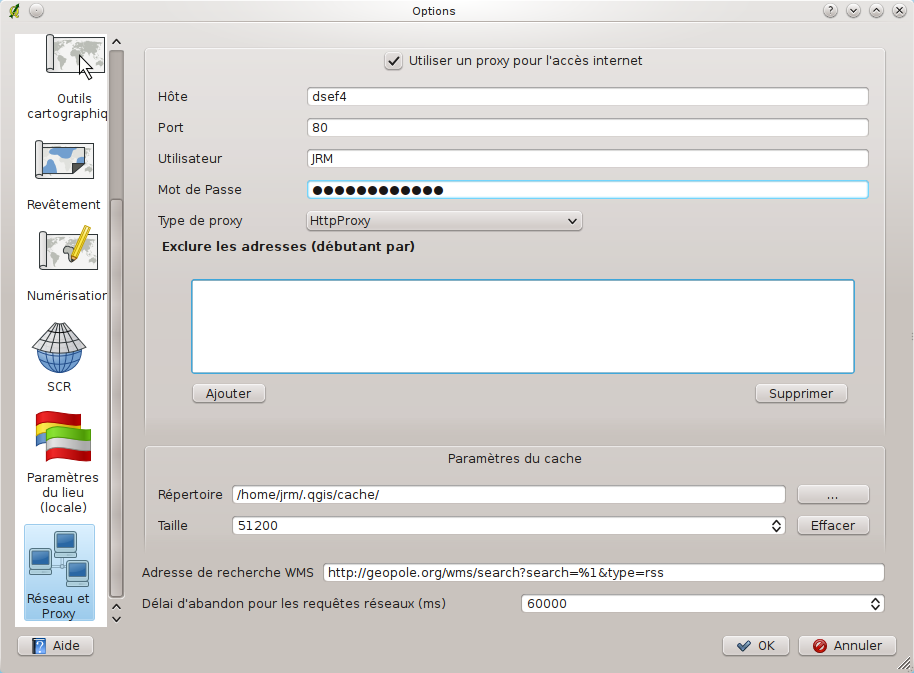
\includegraphics[clip=true, width=10cm]{proxy-settings}
   \label{fig:proxy-settings}
\end{center} 
\end{figure}

\begin{Tip} \caption{\textsc{Usar proxys}}
\qgistip{Usar proxys a veces puede ser complicado. Es útil el 'ensayo y error' con los tipos de proxy anteriores 
y comprobar si son válidos en su caso.
}
\end{Tip}

Puede modificar las opciones de acuerdo con sus necesidades. Algunos 
de los cambios pueden requerir que reinicie QGIS para que tengan efecto.

\begin{itemize}
\item \nix{la configuración se guarda en un archivo de texto: \$HOME/.config/QuantumGIS/qgis.conf}
\item \osx{puede encontrar su configuración en: \$HOME/Library/Preferences/org.qgis.qgis.plist}
\item \win{la configuración se guarda en el registro bajo:}
\begin{verbatim}
\\HKEY\CURRENT\USER\Software\QuantumGIS\qgis
\end{verbatim}
\end{itemize}


\subsection{Marcadores espaciales}\label{sec:bookmarks}
\index{bookmarks}
\index{spatial bookmarks|\see{bookmarks}}

Los marcadores espaciales le permiten ``marcar'' una región geográfica y volver a ella
más tarde.

\subsubsection{Crear un marcador}
Para crear un marcador:
\begin{enumerate}
\item Haga zum o desplácese al área de interés.
\item Seleccione la opción de menú \mainmenuopt{Ver} > \dropmenuopt{Nuevo marcador} o pulse \keystroke{Ctrl-B}.
\item Introduzca un nombre descriptivo para el marcador (hasta 255 caracteres).
\item Pulse \button{Aceptar} para añadir el marcador o \button{Cancelar} para salir sin añadir el marcador.
\end{enumerate}

Tenga en cuenta que puede tener múltiples marcadores con el mismo nombre.

\subsubsection{Trabajar con marcadores}
Para usar o administrar marcadores, seleccione la opción de 
menú \mainmenuopt{Ver} > \dropmenuopt{Mostrar marcadores}.
El diálogo \dialog{Marcadores geoespaciales} le permite hacer zum a un marcador o eliminarlo.
No se puede editar el nombre ni las coordenadas de los marcadores.

\subsubsection{Hacer zum a un marcador}
En el diálogo \dialog{Marcadores geoespaciales} seleccione el marcador deseado y
pínchelo, luego pulse \button{Zum a}. También puede hacer zum a un marcador haciendo
doble clic sobre él.

\subsubsection{Borrar un marcador}
Para borrar un marcador del diálogo \dialog{Marcadores geoespaciales}, pinche en él y luego pulse
 \button{Borrar}.
